\section{Spatiotemporal Features}
In this section, we discuss our proposed spatial features extracted from OpenStreetMap\footnote{\url{https://www.openstreetmap.com}} and temporal features that act as fundamental components of our proposed transfer learning approach. 
Our proposed spatial features capture the traffic-related geographical characteristics for each link in the  road network.

\subsection{Basic Information Features} 
%An example of extracting the basic features indicating the basic information of the link is shown in Figure~\ref{fig:basic}.
We have 5 features for representing the basic information of each link: 
length, \#begin\_node\_in\_links, \#begin\_node\_out\_links, \#end\_node\_in\_links and \#end\_node\_out\_links.
For each link, the \textit{link length} is the real distance between the begin and the end node of this link. 
The number of in and out links connected to both nodes determines the number of in and out links of the two end nodes accordingly.


\subsection{Road Density Features}
Additionally, we believe traffic speed is highly relevant to road density, which can be measured by the number of neighboring nodes and links within the same area.
To be more specific and capture the sensitivity about directions, we compute road density respectively for each end in terms of the density of neighboring node , and the density of neighboring in and out link,  according to three radius (100/300/500m).
%figure:road density feature.
%The nodes in the range of 100, 300 and 500 meters are marked as blue. The in/out links of these nodes are part of link features.
Consequently, we have $2 \times 3 \times 3 = 18$ road density features in total.
%
%\begin{figure}[th!]
%	\centering
%	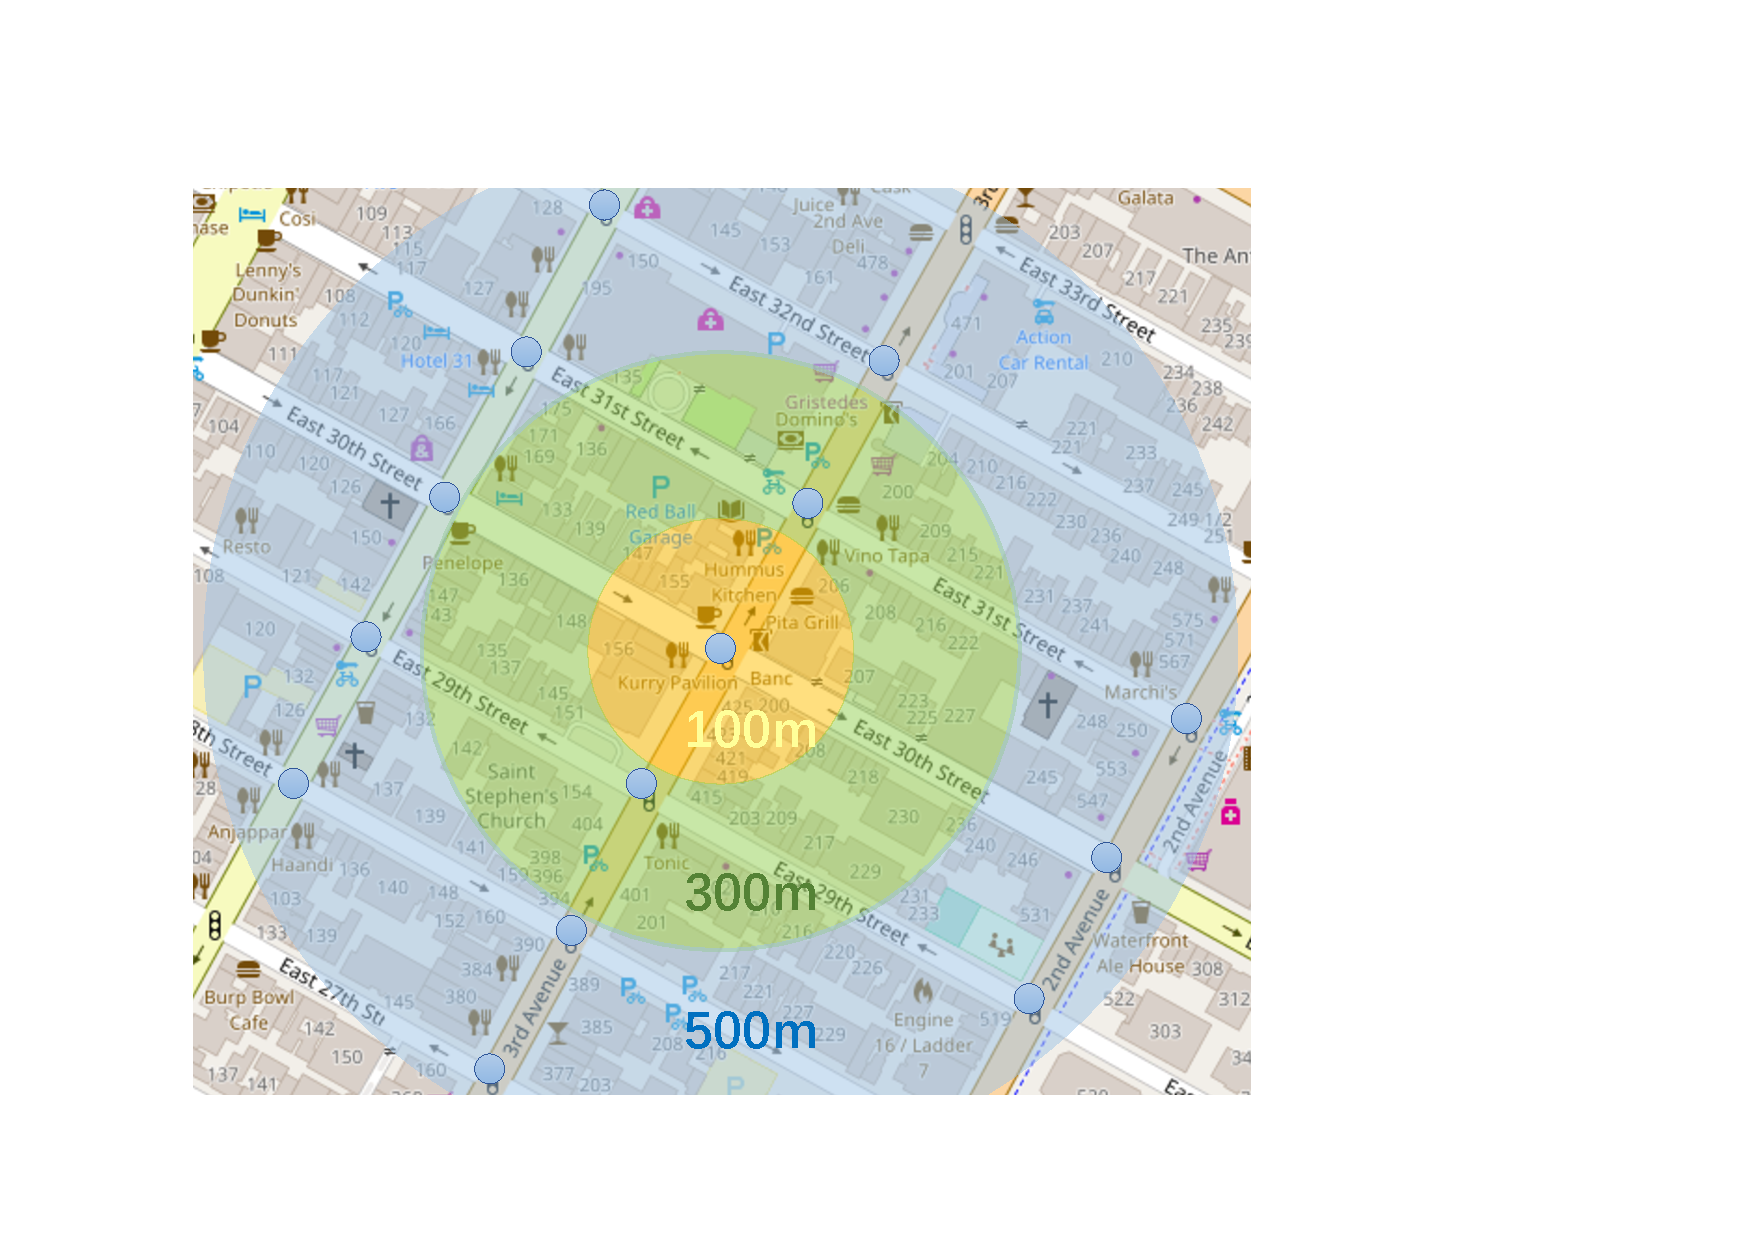
\includegraphics[width=0.45\textwidth]{figures/roaddensity.pdf}
%	\caption{An Example of Extracting the Road Density Features with Three Different Radius with assuming the origin is begin/end node of a certain link}
%	\label{fig:road_density}
%\end{figure}


\subsection{Categorical POI Density Features}
Points of interest (POI) are specific locations that people may find useful or interesting, such as restaurants, shopping halls, parks, etc.
Since such places are very influential to the traffic, we query nearby POIs for each node with three different radius (100/300/500m) using HERE Places API\footnote{\url{https://developer.here.com/documentation/places/topics/introduction.html
}}. 
The POI types we consider are shown in Table~\ref{tbl:poi}.
%The HERE POI category has 83 sub-types and 11 main-types. 
%We merged the sub-types from API responses into main-types. 
%After construction of the features of nodes, the features of links can be derived from them.  
Figure~\ref{fig:poi} shows such an example for extract \textit{road density} features and\textit{ POI density features}.
%\BL{Eve please make a table here to show the 11 main types of POI}


\begin{table}[th]
	\small
	\centering
	\caption{11 Main-types of POI}
	\label{tbl:poi}
	\begin{tabular}{|ccc|}
		\hline
		Eat \& Drink                   & Going Out               & Sights \& Museums \\ 
		Transport                      & Accommodation           & Shopping          \\ 
		Business \& Services           & Facilities              & Facility          \\ 
		Administrative Areas/Buildings & Natural or Geographical &                   \\ \hline
	\end{tabular}
\end{table}


%For each link, the features can be generated from the begin node and the end node. The features of link are divided into three types: basic features, road density features and POI density features. Basic features contain link length and the number of in/out links of begin node and end node. Road density features include the number of following features within three various radius 100, 300 and 500 meters: the number of nearby node and the number of in/out links of these nearby nodes. 


\begin{figure}[th!]
	\centering
	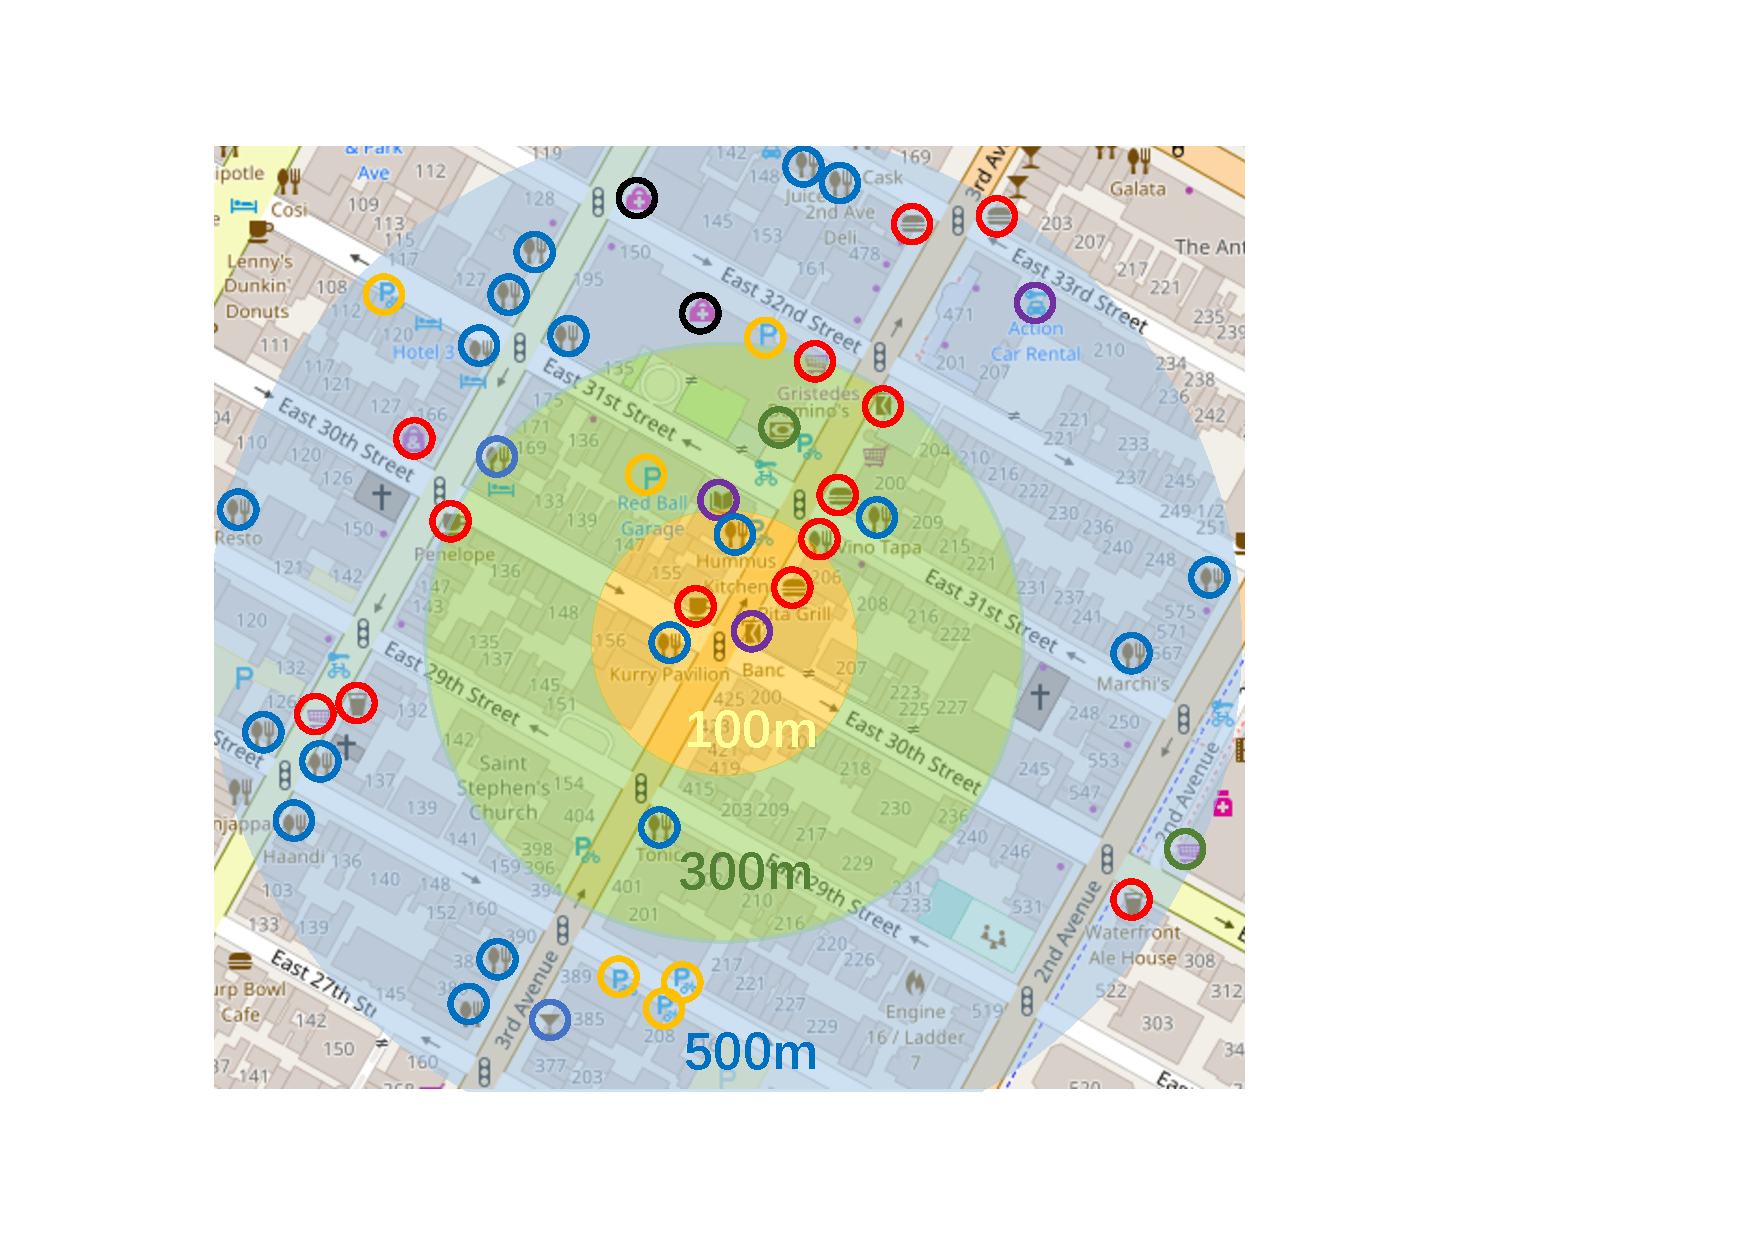
\includegraphics[width=0.55\textwidth]{figures/poi.pdf}
	\caption{An Example of Extracting POI Features. Different colors indicate different POI types.}
	\label{fig:poi}
\end{figure}


\subsection{Temporal Features}
Our temporal feature is simply a distributed representation of the time information.
It is basically a concatenation of several one-hot vectors, 
where each vector represents the \textit{month}, the \textit{day} of a week, the \textit{hour} of a day and whether it is \textit{workday} respectively. 
%To sum up, the total number of spatial and temporal features is 89 and 44 correspondingly.

